%
% $RCSfile: data_and_rules.tex,v $
%
% Copyright (C) 2002-2008. Christian Heller.
%
% Permission is granted to copy, distribute and/or modify this document
% under the terms of the GNU Free Documentation License, Version 1.1 or
% any later version published by the Free Software Foundation; with no
% Invariant Sections, with no Front-Cover Texts and with no Back-Cover
% Texts. A copy of the license is included in the section entitled
% "GNU Free Documentation License".
%
% http://www.cybop.net
% - Cybernetics Oriented Programming -
%
% http://www.resmedicinae.org
% - Information in Medicine -
%
% Version: $Revision: 1.1 $ $Date: 2008-08-19 20:41:06 $ $Author: christian $
% Authors: Christian Heller <christian.heller@tuxtax.de>
%

\paragraph{Data and Rules}
\label{data_and_rules_heading}
\index{Data and Rules}
\index{State- and Logic Knowledge}

Thirdly, \emph{State-} and \emph{Logic} knowledge get distinguished (figure
\ref{statelogic_figure}). It is known from neurological research that the human
brain has special communication regions (optical, acoustical, motoric)
responsible for information input and output. Simply spoken, these regions do
nothing else than translating data, that is an input \emph{State} into an
output \emph{State}, according to special rules which can be summarised by the
term \emph{Logic}.

\begin{figure}[ht]
    \begin{center}
        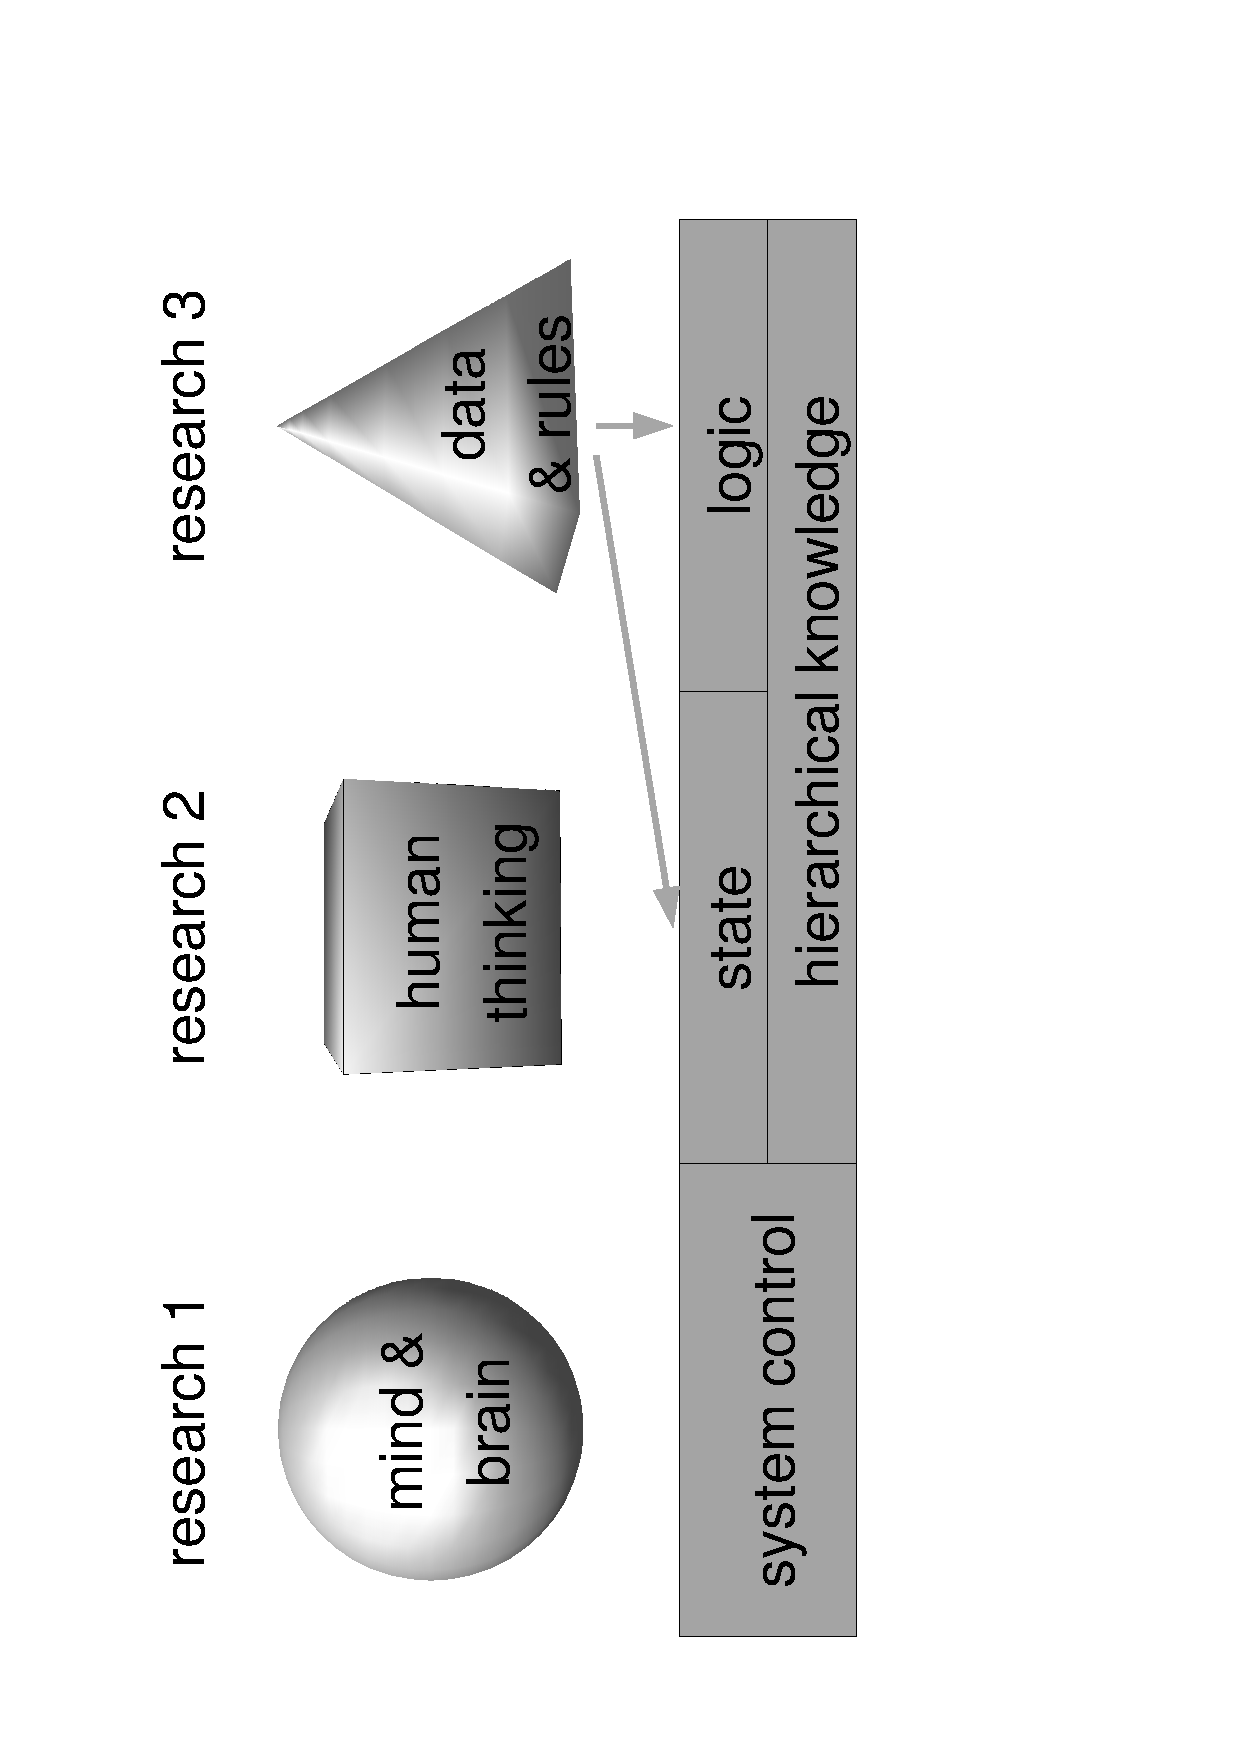
\includegraphics[scale=0.3,angle=-90]{graphic/statelogic.pdf}
        \caption{Translation of Data by Rules Leading to State-/ Logic Knowledge}
        \label{statelogic_figure}
    \end{center}
\end{figure}

This is where systems theory, that uses similar abstractions, comes in. Every
system can be seen as \emph{Black Box} with input/ output (i/o) states and a
translation logic.

When talking about states, this work does \emph{not} mean classical
\emph{State Models} which are often modelled by a \emph{State Chart Diagram}.
A CYBOP state model rather is a composed \emph{Set} of states.

Chapter \ref{state_and_logic_heading} describes more details.
